\documentclass[12pt]{report}

\usepackage[utf8]{inputenc}

\usepackage[dvipsnames]{xcolor}

\usepackage{array}
\newcolumntype{L}{>{\centering\arraybackslash}m{3cm}}

\usepackage{algorithm}
\usepackage{algpseudocode}
\usepackage{caption}

\usepackage{graphicx}
\usepackage{csquotes}

\renewcommand{\bibname}{References}


\title{Advanced Machine Learning\\Final Report}

\author{Shayan Amani}

\date{December 19, 2018}

\begin{document}
\maketitle

\chapter{Problem Definition}
Presenting an optimum policy \cite{Sutton1998} to control a specific invasive species, Frangula alnus, so called glossy buckthorn. For the sake of simplicity, a grid environment of 3x3 has been considered. 

Simulator-generated samples of history of measures and consequences are provided in a dataset. Dataset is consisted of the following columns:
\begin{itemize}
    \item \textbf{V1}: year number of the sample. from 1 to 200 which means simulator run through a span of 200 years.
    \item: \textbf{pop\_1} to \textbf{pop\_9}: population of the plant in each cells.
    \item: \textbf{sbank\_1} to \textbf{sbank\_9}: number of plant's seeds in each cells.
    \item: \textbf{actions}: taken action for each year of samples.
    \item: \textbf{rewards}: observed reward after applying the action.
\end{itemize}

Available actions are defined as a binary set of two actions, $0$ and $10$. Action $0$ means do nothing and action $10$ is equal to cutting and spraying all existing plants in the entire grid.


\chapter{Previous Works}
We have two different point of view to look at this problem. Firstly a batch reinforcement learning problem and secondly invasive species management problem. In retrospect, we can find numerous instances of trying different algorithms and approaches from the community \cite{Phillips2006}, \cite{Phillips2004}, and \cite{Warton2010}.

Such a inter-disciplinary problem is addressed by people active in various fields and they have their own novelties in their points of view. In this report I am elaborating on my approach to the given problem from a relatively new perspective, namely deep reinforcement learning which did not absorb too many attention from the community for presenting solutions to such cases.

\chapter{Method Selection}
As a problem in which the model (transition probabilities) is not provided, model-free design is what may first come to mind. Different options were available to choose among and each have their own pros and cons. From least squares temporal difference (LSTD) \cite{Bradtke1996} or least squares policy iteration (LSPI) \cite{Lagoudakis2003} algorithms to more sophisticated one such as asynchronous advantage actor-critic (A3C) \cite{Mnih2016b} were all available. From a specific perspective, one can point out the diversity among these techniques by a component such as value function approximation technique.

According to the attributes that are observed from the given problem, the final implemented method has been selected. The significant characteristics of the given problem are as follows:
\begin{itemize}
    \item Model is not provided.
    \item Dataset is only a set of generated samples.
    \item Episodic problem.
    \item Inaccessible agent therefore online learning is not possible.
    \item Evidently high correlation between consequent year samples.
\end{itemize}

The mentioned issues are addressed in Chapter \ref{chap: implemented method}

\chapter{Implemented Method}
\label{chap: implemented method}
Considering this sample-based problem I have picked and implemented a deep reinforcement learning approach, namely Deep Q-Networks (DQN). DQN is mostly relied on a stabilization technique with neural networks, called Experience replay \cite{Mnih2015}. The elements of this method are explained in the following sections.

DQN algorithm in a nutshell is a wrapper around Q-learning \cite{Watkins1992}. proposed as an online learning reinforcement learning algorithm, but in this case we need to implement it as a batch learning problem.

One of the method which are excelled in the literature is Deep Deterministic Policy Gradient (DDPG). Such a methods are more applicable to continues action space problems which is not the case here \cite{Lillicrap2015}. I have provided a one-to-one comparison chart in Table \ref{tab:dqn vs. ddpg} to discuss particular aspects of DQN as the implemented method and DDPG as a studied method.


\begin{table}
    \centering
    \begin{tabular}{|c|L|L|L|L|}
        \hline
        \textbf{Method}  &    \textbf{Model Dependence}    &   \textbf{Policy Dependence}   &   \textbf{Action Continuity}  & \textbf{Parent Algorithm(s)}\\
        \hline
        \hline
        DQN &   model-free  &   on-policy   &   discrete    &   Q-learning, DL\\
        \hline
        DDPG    &   model-free  &   on-policy   &   continuous  &   Actor-critic\\
        \hline
    \end{tabular}
    \caption{DRL methods comparison chart}
    \label{tab:dqn vs. ddpg}
\end{table}

\section{Algorithm}
The implemented version of DQN algorithm is described in Algorithm \ref{alg:DQN}. Some variations and consideration are applied to fit this method to the problem.

\begin{algorithm}[H]
\caption{DQN algorithm in batch mode}
\label{alg:DQN}
\begin{algorithmic}[1]
    \State Init D \Comment{\textcolor{BlueViolet}{replay memory}}
    \State Init Q \Comment{\textcolor{BlueViolet}{Q-table w/ random weights}}
    \State \textcolor{OrangeRed}{Get} or Observe $s_0$ \Comment{\textcolor{BlueViolet}{the initial state}}
    \For{each episode}
        \For{samples in each episode}
            \State \textit{\textcolor{OrangeRed}{- skip $\epsilon$-greedy exploration}}
            \State $a = argmax_a Q(s,a)$
            \State \textit{\textcolor{OrangeRed}{- skip applying action $a$ to the environment}}
            \rlap{\smash{$\left.\begin{array}{@{}c@{}}\\{}\\{}\end{array}\color{BlueViolet}\right\}%
              \color{BlueViolet} experience$}}
            \State \textcolor{OrangeRed}{Get} or Observe $r, s'$
            \State Store the \textbf{experience} $<s, a, r, s'>$ in replay memory $D$
            \State \textit{Random} \textbf{sampling} from $D$ $<ss, aa, rr, ss'>$  \Comment{\textcolor{BlueViolet}{[mini]-batch}}
            \If{$ss' \neq $ terminal state} \Comment{\textcolor{BlueViolet}{target for each mini-batch}}
                \State $tt = rr + \gamma max_{aa'} Q(ss', aa')$
            \Else
                \State $tt = rr$
            \EndIf
            \State Train the network
        \EndFor    
    \EndFor
\end{algorithmic}
\end{algorithm}

\section{Neural Network}
The concept of neural networks is a non-linear function approximator \cite{Bengio2009} which approximates action-value function (Q). The inputs to this network are 18 features (9 pop\_i plus 9 sbank\_i) and the outputs are Q-values for two actions 0 and 10. Input, output and hidden layers are selected to be dense (fully-connected) as it doesn't get involved with image processing tasks.

\section{Experience Replay}
DQN is mostly relied on a stabilization technique with neural networks, called Experience replay. Experience replay is a memory abstraction which $n$ past samples are stored in this memory and then we use it later to draw a batch of samples from it on a randomized basis.

Samples are accumulated in the memory while reading from the dataset and within a certain episode.


\section{Random Exploration}
One of the key steps in DQN algorithm is $\epsilon$-greedy exploration. The main purpose of this step is to address exploration-exploitation dilemma. However in this problem we have a batch RL problem and I've skipped this step in the main algorithm.

\section{Results}
Results are provided as dataset which in a policy column is appended. policy says which action should be taken at the end of each year for each episodes. From the loss values observed while training the network and the performance during the run-time, the results seems to be promising. I have also performed a set of measurements on after training like accuracy which shows the method works in operational regions.

% 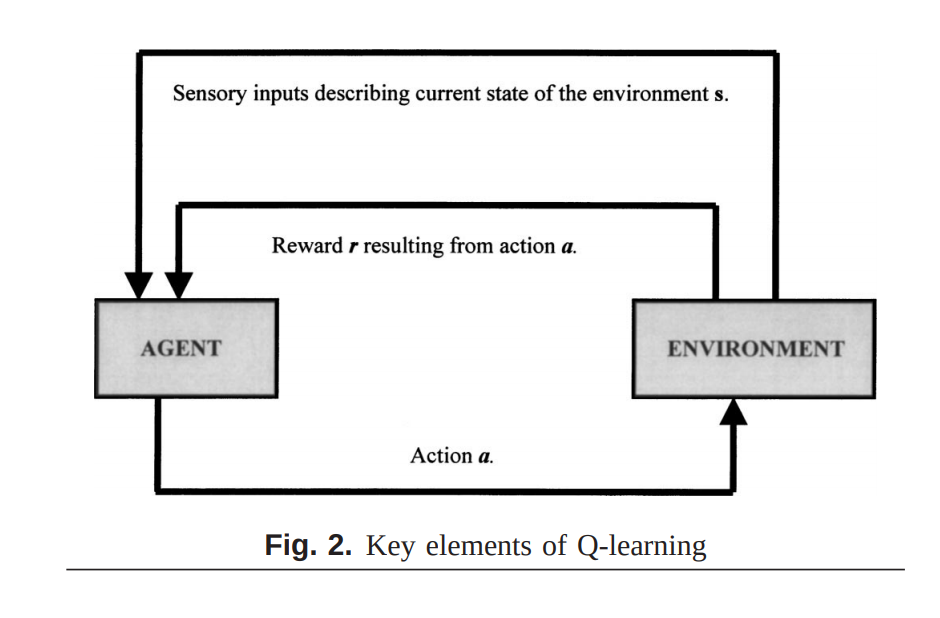
\includegraphics[width=1\columnwidth]{elements.png}

\bibliographystyle{nips}
\bibliography{library}


\end{document}